\documentclass{beamer}


\mode<presentation>
{
  \usetheme{CambridgeUS}
	\usecolortheme{beaver}
  % or ...

  \setbeamercovered{transparent}
  % or whatever (possibly just delete it)
}


\usepackage{xeCJK}
\usepackage{ulem}
\usepackage[english]{babel}
\usepackage[utf8]{inputenc}
\usepackage{times}
\usepackage[T1]{fontenc}
\usepackage{hyperref}
\usepackage{pifont}
\usepackage{biblatex}
\usepackage{bibentry}
\usepackage{verbatim}
\usepackage{listings}
\bibliography{cite}
\newcommand{\cmark}{\ding{51}}%
\newcommand{\xmark}{\ding{55}}%
\setCJKmainfont{WenQuanYi Micro Hei}
\renewcommand{\raggedright}{\leftskip=0pt \rightskip=0pt plus 0cm}
\raggedright

\let\oldfootnotesize\footnotesize
\renewcommand*{\footnotesize}{\oldfootnotesize\tiny}

\title[Intelligent Software Engineering] 
{Intelligent Software Engineering}
\subtitle{Requirements Engineering}

\author[Zhilei Ren] 
{Zhilei Ren}

\institute[Dalian University of Technology] % (optional, but mostly needed)
{
\\
\includegraphics[width=0.1\textwidth]{../utils/logo.png}\\
Dalian University of Technology
}


\subject{Software Engineering}



\pgfdeclareimage[width=0.08\textwidth]{university-logo}{../utils/logo.png}
\logo{\pgfuseimage{university-logo}}



% Delete this, if you do not want the table of contents to pop up at
% the beginning of each subsection:
\AtBeginSubsection[]
{
  \begin{frame}<beamer>{Outline}
    \tableofcontents[currentsection,currentsubsection]
  \end{frame}
}


% If you wish to uncover everything in a step-wise fashion, uncomment
% the following command: 

%\beamerdefaultoverlayspecification{<+->}

\setbeamertemplate{section in toc}[circle]
\setbeamertemplate{items}[circle]
\setbeamertemplate{caption}[numbered]
\setbeamertemplate{bibliography item}{\insertbiblabel}
\setbeamertemplate{bibliography entry title}{}
\setbeamertemplate{bibliography entry journal}{}

% PlantUML listing configuration
\lstdefinestyle{plantuml}{
    language=Java,
    basicstyle=\ttfamily\small,
    keywordstyle=\color{blue},
    commentstyle=\color{green!60!black},
    stringstyle=\color{red},
    numbers=left,
    numberstyle=\tiny\color{gray},
    stepnumber=1,
    numbersep=5pt,
    backgroundcolor=\color{white!95!black},
    frame=single,
    rulecolor=\color{black},
    tabsize=2,
    captionpos=b,
    breaklines=true,
    breakatwhitespace=false,
    showstringspaces=false
}

\begin{document}

\begin{frame}
  \titlepage
\end{frame}

%\begin{frame}{Outline}
%  \tableofcontents[currentsection,currentsubsection, 
%    hideothersubsections, 
%    sectionstyle=show,
%]
%\end{frame}

\AtBeginSection[]
{
 \begin{frame}<beamer>
 \frametitle{Outline}
 \tableofcontents[currentsection]
 \end{frame}
}
\begin{frame}[t]{Definition of Requirements Engineering}
    Requirements engineering is an interdisciplinary function that mediates between the domains of the acquirer and supplier or developer to establish and maintain the requirements to be met by the system, software or service of interest. Requirements engineering is concerned with discovering, eliciting, developing, analyzing, verifying (including verification methods and strategy), validating, communicating, documenting and managing requirements\footnote{ISO/IEC/IEEE 29148 Systems and software engineering — Life cycle processes -- Requirements engineering}.
\end{frame}

\begin{frame}[t]{As Proposed by the Project Sponsor}
    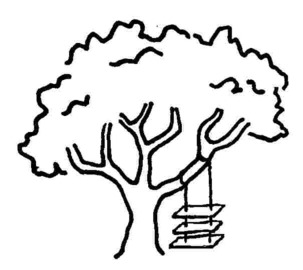
\includegraphics[width=.4\textwidth]{treemark.jpg} 
\end{frame}

\begin{frame}[t]{As Specified in the Project Request}
    
\includegraphics[width=.4\textwidth]{treemana.jpg} 
\end{frame}
\begin{frame}[t]{As Designed by the Senior Systems Analyst}
    
\includegraphics[width=.4\textwidth]{treeeng.jpg} 
\end{frame}
\begin{frame}[t]{As Produced by the Programmers}
    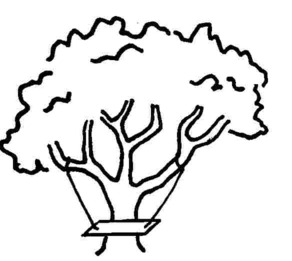
\includegraphics[width=.4\textwidth]{treemanu.jpg} 
\end{frame}
\begin{frame}[t]{As Installed at the User's Site}
    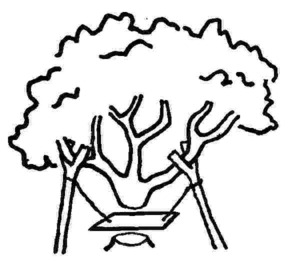
\includegraphics[width=.4\textwidth]{treemain.jpg} 
\end{frame}
\begin{frame}[t]{What The User Wanted}
    
\includegraphics[width=.4\textwidth]{treecust.jpg}
\end{frame}

\begin{frame}[t]{Guide to Good Programming Practice, 1979}
    
\includegraphics[width=.4\textwidth]{treeswing_computer_book_cover.jpg}
\end{frame}

\begin{frame}[t]{Research Topics in Requirements Engineering}
    \begin{enumerate}
        \item Requirements Classification
        \item Requirements Prioritization
        \item Feature Model Optimization
        \item Prototype Generation
    \end{enumerate}
\end{frame}

\begin{frame}[t]{Techniques for Requirements Engineering Research}
\end{frame}

\begin{frame}[t]{Next Release Problem}
    % https://mde-optimiser.github.io/case-studies/nrp/
    % https://www.sciencedirect.com/science/article/pii/S095058490100194X
    % feature model
    Given:
    \begin{itemize}
      \item A set of software requirements \( R = \{r_1, r_2, \dots, r_n\} \),
      \item A set of customers \( C = \{c_1, c_2, \dots, c_m\} \),
      \item Each customer \( c_j \in C \) requests a subset of requirements \( R_j \subseteq R \) and provides a profit  \( p_j > 0 \) if all requirements in \( R_j \) are satisfied,
      \item Each requirement \( r_i \in R \) has an associated cost \( \text{cost}(r_i) > 0 \),
      \item A total available budget \( B > 0 \).
    \end{itemize}

    The goal is to select a subset of requirements \( R' \subseteq R \) such that:
    \begin{enumerate}
      \item The total cost does not exceed the budget: $\sum_{r_i \in R'} \text{cost}(r_i) \leq B$, 
      \item The total profit is maximized:
      \[
      \max_{R' \subseteq R} \sum_{\substack{c_j \in C \\ R_j \subseteq R'}} p_j.
      \]
    \end{enumerate}

    This is known as the \textbf{Next Release Problem (NRP)} and is a well-known NP-hard problem in requirements engineering and software release planning.
\end{frame}

\begin{frame}[t]{bug or feature?}
    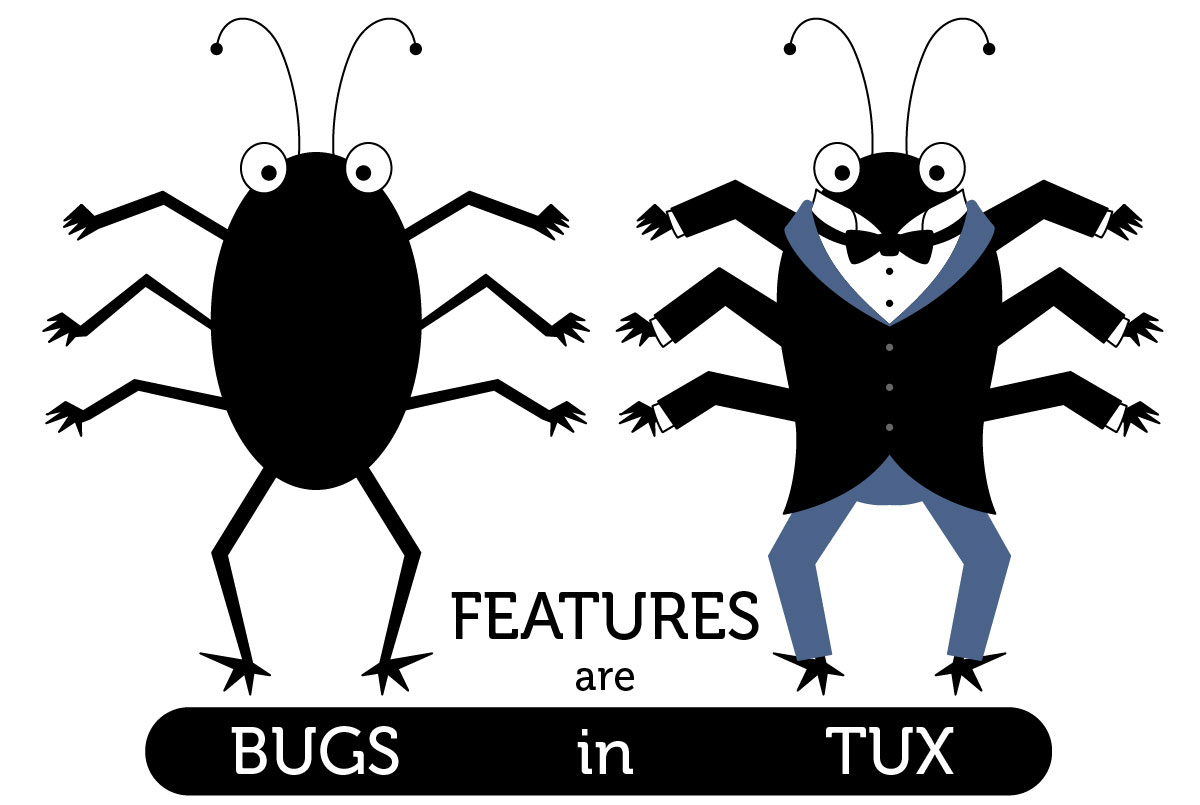
\includegraphics[width=.5\textwidth]{bugfeature.jpg}
\end{frame}
\begin{frame}[t]{The First Computer Bug}
    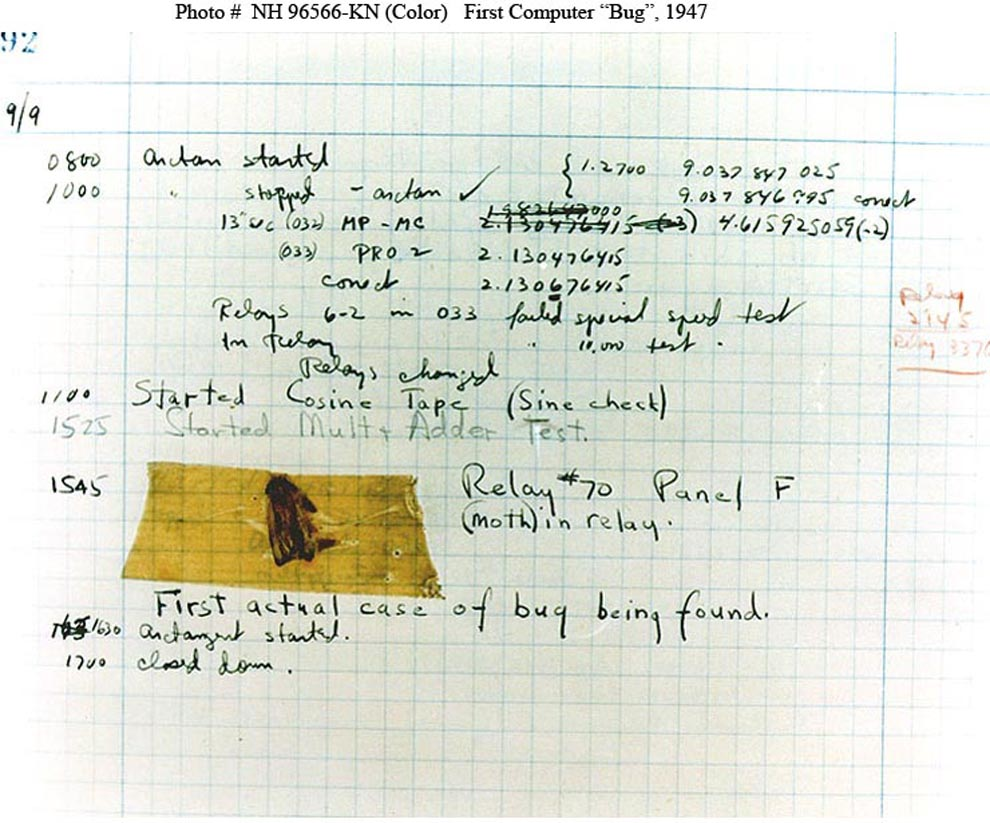
\includegraphics[width=.5\textwidth]{computer-bug.jpg}  
\end{frame}
\begin{frame}[t]{The First Computer Bug}
    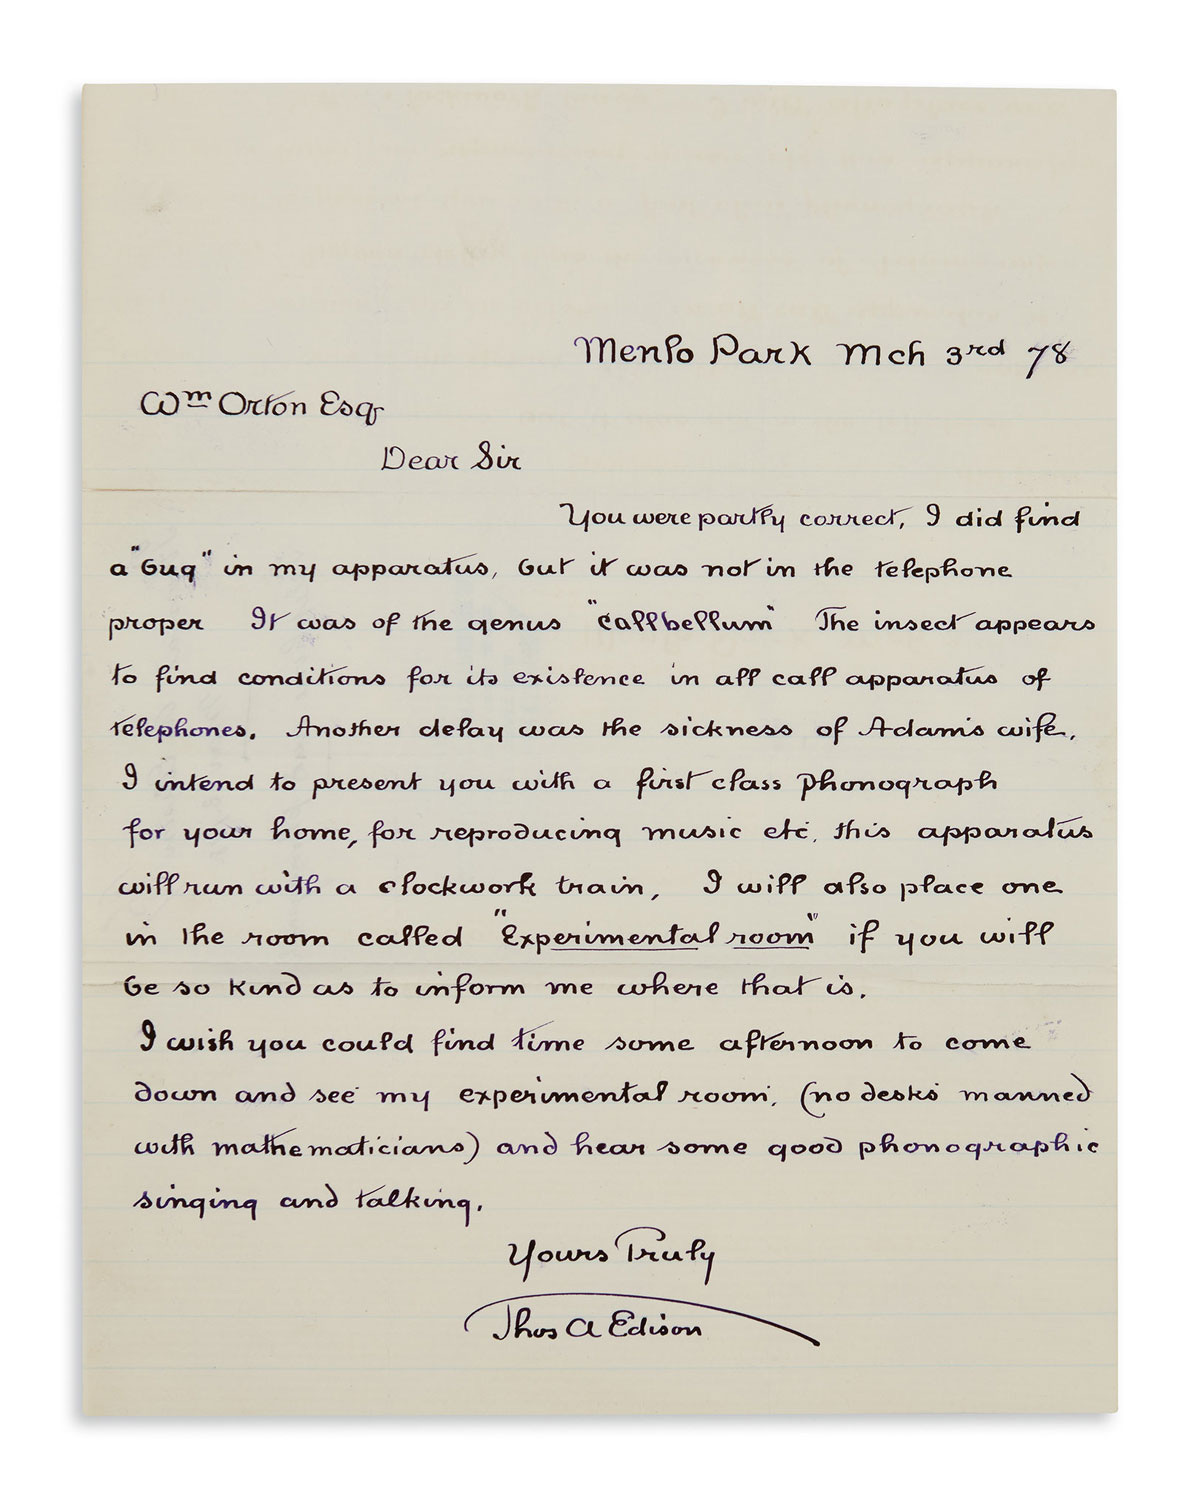
\includegraphics[width=.5\textwidth]{telebug.jpg}  
\end{frame}
\begin{frame}[t]{Combo}
    Combos were a design accident; lead producer Noritaka Funamizu noticed that extra strikes were possible during a bug check on the car-smashing bonus stage. He thought that the timing required was too difficult to make it a useful game feature, but left it in as a hidden one\footnote{\url{https://en.wikipedia.org/wiki/Combo_(video_games)}}.

    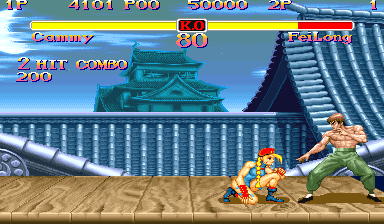
\includegraphics[width=.5\textwidth]{Super_Street_Fighter_II_screenshot.png}

\end{frame}

\begin{frame}[t]{彩蛋}
    
\includegraphics[width=.5\textwidth]{1280px-Konami_Code.svg.png} 
\end{frame}

\section{PlantUML}

% Slide 1: What is PlantUML?
\begin{frame}{What is PlantUML?}
    \begin{itemize}
        \item \textbf{Definition:} Open-source tool for creating diagrams from plain text descriptions
        \item \textbf{Core Idea:} Uses simple, human-readable Domain Specific Language (DSL)
        \item \textbf{Foundation:} Java-based tool leveraging Graphviz for layout
        \item \textbf{Philosophy:} Focus on content rather than manual layout
    \end{itemize}
    
    \begin{quote}
        "PlantUML is a versatile component for quickly and directly creating diagrams."
    \end{quote}
\end{frame}

% Slide 2: Key Advantages
\begin{frame}{Key Advantages}
    \begin{table}
    \small
    \begin{tabular}{p{0.4\textwidth} p{0.55\textwidth}}
    \textbf{Advantage} & \textbf{Description} \\
    \hline
    Version Control Friendly & Text files work with Git - enables change history, diffing, collaboration \\
    Efficiency \& Speed & Faster than manual graphical editing, especially for complex diagrams \\
    Maintainability \& Consistency & Easy updates and consistent styling with themes \\
    Automation \& Integration & Integrates with documentation pipelines, build systems, CI/CD \\
    \end{tabular}
    \end{table}
\end{frame}

% Slide 3: UML Diagrams Supported
\begin{frame}{UML Diagrams Supported}
    \begin{columns}
    \begin{column}{0.5\textwidth}
        \begin{itemize}
            \item Sequence Diagram
            \item Use Case Diagram
            \item Class Diagram
            \item Activity Diagram
            \item Component Diagram
            \item Deployment Diagram
            \item State Diagram
            \item Object Diagram
        \end{itemize}
    \end{column}
    \begin{column}{0.5\textwidth}
        \centering
        \textbf{Visual Example:}\\
        \textcolor{gray}{\scriptsize[Diagram placeholder]}
        \vspace{2cm}
    \end{column}
    \end{columns}
\end{frame}

% Slide 4: Beyond UML
\begin{frame}{Beyond UML Diagrams}
    \begin{itemize}
        \item Architectural Diagrams (C4 model)
        \item Entity Relationship Diagrams (ERD)
        \item Wireframes / UI Mockups (salt library)
        \item Gantt charts for project management
        \item Mind Maps for brainstorming
        \item JSON/YAML visualization
        \item Network diagrams
    \end{itemize}
\end{frame}

% Slide 5: How It Works
\begin{frame}{How PlantUML Works}
    \begin{enumerate}
        \item \textbf{Write:} Create text file (.puml) with PlantUML syntax
        \item \textbf{Process:} Java processor parses text, converts to Graphviz DOT language
        \item \textbf{Render:} Layout engine generates final image
        \item \textbf{Output:} Get image in desired format (PNG, SVG, etc.)
    \end{enumerate}
    
    \begin{center}
    \textbf{Text} $\rightarrow$ \textbf{PlantUML} $\rightarrow$ \textbf{Graphviz} $\rightarrow$ \textbf{Diagram}
    \end{center}
\end{frame}

% Slide 6: Sequence Diagram Example
\begin{frame}[fragile]{Syntax Example: Sequence Diagram}
    \begin{lstlisting}[style=plantuml]
@startuml
actor User
participant "Web Browser" as Browser
participant Server

autonumber
User -> Browser: Enter URL
Browser -> Server: HTTP Request
Server -> Server: Process Request
Server --> Browser: Return HTML
Browser --> User: Display Page
@enduml
    \end{lstlisting}
    
    \small
    \begin{itemize}
        \item \texttt{@startuml/@enduml}: Diagram boundaries
        \item \texttt{actor}, \texttt{participant}: Element declarations
        \item \texttt{->}, \texttt{-->}: Solid/dashed arrows
        \item \texttt{autonumber}: Automatic message numbering
    \end{itemize}
\end{frame}

% Slide 7: Use Case Diagram Example
\begin{frame}[fragile]{Syntax Example: Use Case Diagram}
    \begin{lstlisting}[style=plantuml]
@startuml
left to right direction
actor "Library User" as User
usecase "Borrow Book" as Borrow
usecase "Search Catalog" as Search

User --> Borrow
User --> Search
@enduml
    \end{lstlisting}
    
    \small
    \begin{itemize}
        \item \texttt{left to right direction}: Layout control
        \item \texttt{actor}, \texttt{usecase}: Actor and use case definitions
        \item \texttt{-->}: Connection arrows
    \end{itemize}
\end{frame}

% Slide 8: Getting Started
\begin{frame}{Getting Started with PlantUML}
    \textbf{Online Servers (Quick Start):}
    \begin{itemize}
        \item Official server: \href{http://plantuml.com}{plantuml.com}
        \item Community site: \href{http://planttext.com}{planttext.com}
        \item No installation required
    \end{itemize}
    
    \vspace{0.5cm}
    \textbf{Local Installation (Recommended):}
    \begin{itemize}
        \item Prerequisites: Java JRE + Graphviz
        \item IDE Plugins: VSCode, IntelliJ, Eclipse
        \item Command Line: Use \texttt{plantuml.jar}
    \end{itemize}
\end{frame}

% Slide 9: Summary
\begin{frame}{Summary \& Key Takeaways}
    \begin{itemize}
        \item \textbf{Why PlantUML?} Version control, automation, efficiency
        \item \textbf{Text-Based:} Simple, readable language for diagrams
        \item \textbf{Wide Support:} Comprehensive UML + additional diagram types
        \item \textbf{Easy Integration:} Fits modern development workflows
        \item \textbf{Quick Start:} Online editors → local integration
    \end{itemize}
    
    \vspace{0.5cm}
    \textbf{Embrace efficient diagram creation and maintenance!}
\end{frame}

% Final slide
\begin{frame}
    \frametitle{Thank You \& Questions}
    
    \begin{center}
    \Large
    \textbf{Resources}
    \end{center}
    
    \vspace{0.5cm}
    \begin{itemize}
        \item Official Website: \href{http://plantuml.com}{plantuml.com}
        \item Online Demo: \href{http://plantuml.com/plantuml}{plantuml.com/plantuml}
        \item Documentation: \href{http://plantuml.com/guide}{plantuml.com/guide}
    \end{itemize}
    
    \vspace{1cm}
    \begin{center}
    \large
    Questions?
    \end{center}
\end{frame}

\end{document}

